\documentclass[french, a4paper]{beamer}
\usepackage{url}
\usepackage{hyperref}
\hypersetup{%
    hidelinks,
    pdfinfo = {%
        Author = {Paul Mabileau},
        Title = {Soutenance de Mission en Entreprise},
        Subject = {Stage de fin d'études},
        Keywords = {%
            présentation,
            stage,
            ingénieur,
            intégration,
            sécurité,
            OCD,
            Orange Cyberdéfense,
        },
    },
}

\usepackage[french]{babel}
\usepackage[utf8x]{inputenc}
\usepackage{times}
\usepackage{beamerthemeWarsaw}
\usepackage{caption}
\usepackage{subcaption}
% \usetheme{Berlin}
\usecolortheme{seagull}
\usefonttheme{serif}
\useoutertheme{shadow}
% \useinnertheme{rectangles}

\captionsetup{justification = centering}
\setbeamertemplate{navigation symbols}{}
\setbeamerfont{page number in head/foot}{size = \small}
\setbeamertemplate{footline}{%
    \hspace{0.2cm}
    \vspace{0.2cm}
    \insertframenumber{} / \inserttotalframenumber{}
}

\captionsetup[figure]{labelformat = empty}
\logo{
\includegraphics[height = 15mm]{img/logo/tsp.png}}

\AtBeginSection[] {%
    \begin{frame}
        \tableofcontents[
            currentsection,
            sectionstyle = show/shaded,
            subsectionstyle = show/show/hide,
            subsubsectionstyle = hide/hide/hide/hide,
        ]{}
    \end{frame}
}

\AtBeginSubsection[] {%
    \begin{frame}
        \tableofcontents[
            currentsection,
            sectionstyle = show/hide,
            subsectionstyle = show/shaded/hide,
            subsubsectionstyle = show/show/hide/hide,
        ]{}
    \end{frame}
}


\title{Soutenance de stage: Orange Cyberdéfense}
\subtitle{Intégration sécurité}
\author{Paul Mabileau}
\institute{Télécom SudParis}
\date{7 Octobre 2021}



\begin{document}


\begin{frame}
    \titlepage{}
\end{frame}

\begin{frame}
    \begin{center}
        {\Large Plan}
    \end{center}
    \tableofcontents[subsubsectionstyle = hide]
\end{frame}


\section{Introduction}
\subsection{Stage}

\begin{frame}
    \frametitle{Intégration}
    \begin{figure}[h!]
        \centering
        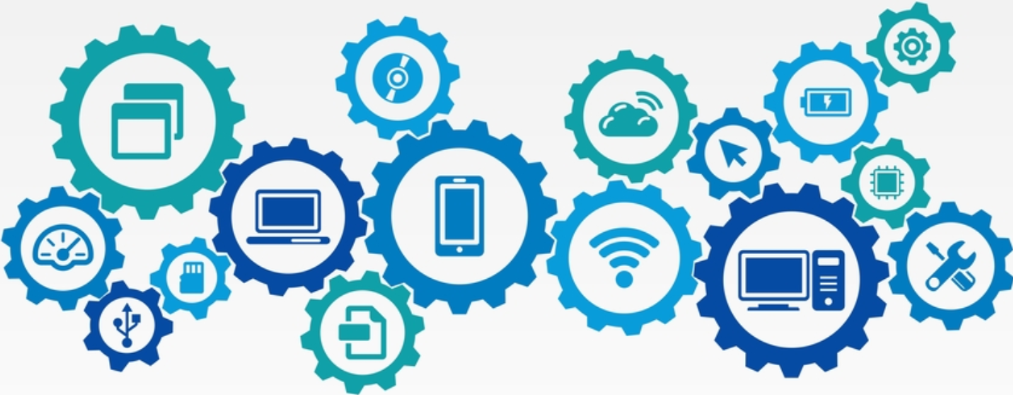
\includegraphics[width = \linewidth]{img/misc/integ.png}
        \caption{Intégration de système}%
        \label{fig:misc/integ}
    \end{figure}
\end{frame}

\subsection{Présentation de l'entreprise}

\begin{frame}
    \frametitle{Orange Cyberdéfense}
    \begin{minipage}{0.5\textwidth}
        \begin{itemize}
            \item Filiale d'Orange Business Services et du groupe Orange.
            \item Fondée en 2014, marque créée en 2016, 1100 employés.
            \item Fournit divers services de sécurité informatique.
        \end{itemize}
    \end{minipage}%
    \hfill
    \begin{minipage}{0.5\textwidth}
        \begin{figure}[h!]
            \centering
            
\includegraphics[width = \linewidth]{img/logo/ocd.png}
            \caption{Logo de l'entreprise}%
            \label{fig:logo/ocd}
        \end{figure}
    \end{minipage}
\end{frame}


\section{Mission}
\subsection{Objectifs}
\subsection{Premières missions}
\subsection{Deuxième mission: projet SNCF}
\subsection{Mission principale: projet Hynamics}
\subsubsection{Considérations générales}
\subsubsection{Démarrage et premières opérations}
\subsubsection{Collecte des informations et déploiement sur sites}
\subsubsection{Implémentation de la configuration}
\subsubsection{Mise en place des tests et migration}
\subsubsection{Transferts de connaissances}


\section{Bilan}
\subsection{Retour d'expérience}


\section{Conclusion}
\subsection{Perspectives}


\end{document}
